\section{UNBALANCED OPTIMAL TRANSPORT SCREENING}
\subsection{Screening for UOT}

We can get the dual form of the UOT problem: 
For $d(\mat{X} \vec{t}) = \frac{1}{2}\|\mat{X} \vec{t}-\vec{y}\|_2^2$, the dual Lasso problem has the following form:
 \begin{equation}
\begin{split} 
d^*(-\theta) = \frac{1}{2}\|\theta\|_2^2-\vec{y}^{\tranT}\theta
 \end{split}
\end{equation}

 \begin{equation}
\begin{split} 
g^*(\mat{X}^{\tranT}\theta) = \left\{
\begin{aligned}
0 \quad&\quad ( \forall \vec{t} \quad\theta^{\tranT}\mat{X}\vec{t} - g(\vec{t}) \leq 0 )\\
\infty \quad&( \exists t \quad\theta^{\tranT}\mat{X}\vec{t} - g(\vec{t}) \leq 0 )
\end{aligned}
\right.
 \end{split}
\end{equation}

For UOT problem \ref{eq:uot}, we could get its dual form. 
\begin{lem}(Dual form of UOT problem)
\begin{equation}
\begin{split}
-d^*(-\theta) - g^*(\mat{X}^{\tranT}\theta)& = -\frac{1}{2}\|\theta\|_2^2-\vec{y}^{\tranT}\theta \\
 \mathbf{s.t.} \quad \forall p \quad \vec{x}_p^{\tranT}\theta -\lambda \vec{c}_p &\leq 0
 \end{split}
 \label{eq:uotdual}
\end{equation}
\end{lem}
$\vec{x}_p $ is the p-th column of $\mat{X}$, It is clear that the strongly concave coefficient $L$ for the dual function $d$ is 1. These inequations \ref{eq:uotdual} make up a dual feasible area written as $\mathcal{R}^{D}$, and the optimal solution satisfied them.\\
From the KKT condition, we know that for the optimal primal solution $\hat{\vec{t}}$:
\begin{thm} (KKT condition) For the dual optimal solution $\hat{\theta}$, we have the following relationship:
 \begin{equation}
\begin{split}
\vec{x}_p^{\tranT}\hat{\theta} -\lambda \vec{c}_p \left\{
\begin{aligned}
< 0 \quad& \Rightarrow \hat{\vec{t}}_p = 0\\
= 0 \quad& \Rightarrow \hat{\vec{t}}_p \geq 0
\end{aligned}
\right.
 \end{split}
 \label{eq:kkt}
\end{equation}
\end{thm}

\ref{eq:kkt} indicates to us a potential method to screening the primal variable, as we do not know the information of $\hat{\vec{t}}$ directly, we construct an area $\mathcal{R}^{S}$ containing the $\hat{\vec{t}}$, if

\begin{equation}
\max_{\vec{t} \in \mathcal{R}^S} \vec{x}_p^{\tranT}\theta -\lambda \vec{c}_p < 0
\end{equation}
then we have:
 \begin{equation}
 \vec{x}_p^{\tranT}\hat{\theta} -\lambda \vec{c}_p < 0 
 \label{eq:kktineq}
\end{equation}
which means the corresponding $\hat{t}_p = 0$, and can be screened out.
As for the UOT problem, $x_p = [...,0,1,0,...,0,1,0,...,]^{\tranT}$, which has only two elements $p_1$, $p_2$ equal to 1, we can set $\theta = [\vec{u}^{\tranT},\vec{v}^{\tranT}]^{\tranT}$ and $\vec{u}\in\R^{m}, \vec{v}\in\R^{n}$, assuming $p=(I,J), I = p \mid m, J = p \mod m$. then we could rewrite \ref{eq:kktineq} as 

 \begin{equation}
\vec{u}_{I} + \vec{v}_{J}-\lambda \vec{c}_p < 0
\end{equation}

Before we start to construct the area containing $\hat{\theta}$, from \ref{circle} we know that we have to find a $\tilde{\theta}$ in the dual feasible area $\mathcal{R}^{D}$ firstly, there is a relationship between the primal variable and dual variable $\theta = \vec{y} - \mat{X}\vec{t}$, however, sometimes the outcome $\theta \notin \mathcal{R}^{D}$, which asks us to project. In the lasso problem, as the constraints limit the $\|\vec{x}_p \theta\|_1$, and every element of $\theta$ is multiplied by a dense $x_i$, researchers have to use a shrinking method to obtain a $\tilde{\theta} \in \mathcal{R}^{D}$ for further constructing the dual screening area: 
\begin{equation}
\tilde{\theta} = \frac{\lambda \vec{c} ^{\tranT}(\vec{y} - \mat{X} \vec{t})}{\max(\lambda \vec{c}, \|\mat{X}^{\tranT}(\vec{y}-\mat{X}\vec{t})\|_{\infty})}
\end{equation}
Unlike in the Lasso problem, This method pushes the $\theta$ far away from the optimum $\hat{\theta}$ and can not work when one of the costs $\vec{c}_p = 0$, which never happens in the Lasso problem but frequently in the UOT problem. The whole dual elements would degenerate to zero and disable the screening process. As for the UOT problem, it only allows $\vec{t}_p \geq 0$, and the $x_p$ only consists of two non-zero elements, which allows us to adapt a better projection method:

\begin{thm}
(UOT shifting projection) For any $\theta = [{\vec{u}}^{\tranT},{\vec{v}}^{\tranT}]^{\tranT}$, we can compute the projection $\tilde{\theta} = [\tilde{\vec{u}}^{\tranT},\tilde{\vec{v}}^{\tranT}]^{\tranT} \in \mathcal{R}^{D}$ by.
\begin{equation}
\begin{split}
\tilde{\vec{u}}_I &= {\vec{u}}_I - \max_{0\geq j\geq n} \frac{{\vec{u}}_I +{\vec{v}}_j - \lambda\vec{c}_{p}}{2}\\
& = \frac{{\vec{u}}_I +\lambda\vec{c}_{p}}{2} - \frac{1}{2}\max_{0\geq j\geq n} {\vec{v}}_j\\
\tilde{\vec{v}}_J &= {\vec{v}}_J - \max_{0 \geq i \geq m} \frac{{\vec{u}}_i +{\vec{v}}_J - \lambda\vec{c}_{p}}{2}\\
& = \frac{{\vec{v}}_J +\lambda\vec{c}_{p}}{2} - \frac{1}{2}\max_{0\geq i\geq m} {\vec{u}}_j
 \end{split}
 \label{eq:uotproj}
\end{equation}
\end{thm}
	\begin{figure}[h]
	\begin{center}	
	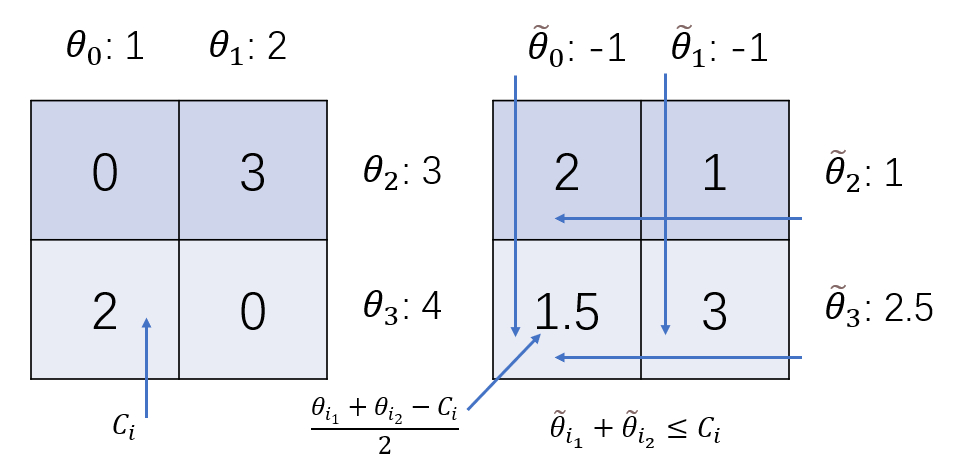
\includegraphics[width = \linewidth]{pic/shifting}
	\caption{Shifting on a 2$\times$2 matrix}
	\end{center}	
	\end{figure}


As we have got the $\tilde{\theta}$ in the $R^{D}$ and we also have another constraint area $\mathcal{R}^{C}$, we are sure that the $\hat{\vec{t}} \in \mathcal{R}^{C}\cap\mathcal{R}^{D}$. However, The intersection of a sphere and a polytope can not be computed in $O(knm)$, where $k$ is a constant. We design a relaxation method. which divides the constraints into two parts, then we maximize the intersection of two hyperplanes and a hyper-ball. 

	\begin{figure}[h]
	\begin{center}	
	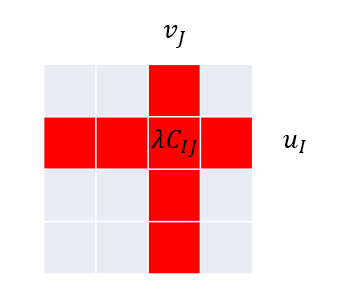
\includegraphics[width = \linewidth]{pic/divide}
	\caption{Selection of group $A_{IJ}$(red) and $B_{IJ}$(grey)}
	\end{center}	
	\end{figure}

\begin{thm}\label{area}(Two plane Screening for UOT) For every single primal variable $t_p$, let $A_p = \{ i \| 0\leq i<nm, i\mid m = I \vee i\mod m = J\}$, $B_p = \{ i \| 0\leq i<nm, i \notin A_p\}$. we can construct the specific area $\mathcal{R}^{S}_{IJ}$ for it.
 \begin{equation}
\begin{split} 
\mathcal{R}^S_{IJ} = \{\theta \|
\begin{aligned}
 &\sum_{l\in A_p}(\theta^{\tranT}\vec{x}_{l}\vec{t}_l - \lambda \vec{c}_l \vec{t})\leq 0 \\
 &\sum_{l\in B_p}(\theta^{\tranT}\vec{x}_{l}\vec{t}_l - \lambda \vec{c}_l \vec{t})\leq 0 \\
  &(\theta-\tilde{\theta})^{\tranT}(\theta-\vec{y})\leq 0
\end{aligned}
\}
\end{split}
\label{eq:divide}
\end{equation}
\end{thm}
We divide the constraints into two groups $A_p$ and $B_p$ for every single $p$, this problem can be solved easily by the Lagrangian method in constant time, the computational process is in Appendix. A


\subsection{Screening Algorithms}

 \begin{algorithm}
 \caption{UOT Dynamic Screening Algorithm}
 \begin{algorithmic}[h]
 \renewcommand{\algorithmicrequire}{\textbf{Input:}}
 \renewcommand{\algorithmicensure}{\textbf{Output:}}
 \REQUIRE $\vec{t}_0, S \in R^{n\times m}, S_{ij}=1, (i,j) = mi+j$
 \ENSURE $S$
 \STATE \text{Choose a solver for the problem.}
 \FOR {$k = 0 \text{ to } K$}
 \STATE $\text{Projection } \tilde{\theta} = \operatorname{Proj}(t^k)$ 
 \FOR {$i = 0 \text{ to } m$}
  \FOR {$j = 0 \text{ to } n$}
  \STATE $\mathcal{R}^{S} \Leftarrow \mathcal{R_{ij}}^S{(\tilde{\theta},t^k)}$
   \STATE $S \Leftarrow {S_{ij} = 0 \text{ if } \max_{\theta \in \mathcal{R}^S} {x_{(i,j)}}^{\tranT}\theta <\lambda c_{(i,j)} }$
 \ENDFOR
  \ENDFOR
 \FOR {$(i,j) \in \{(i,j)\|S_{ij}=0\}$}
  \STATE $\vec{t}^k_{(i,j)} \Leftarrow 0$
  \ENDFOR
  \STATE $\vec{t}^{k+1} = \operatorname{update}(\vec{t}^k)$
 \ENDFOR
  
 \RETURN $\vec{t}^{K+1}, S $ 
 \end{algorithmic} 
 \end{algorithm}

The screening method is irrelevant to the optimization solver you choose. We give the specific algorithm for $L_2$ UOT problem to show the whole optimization process. The $\operatorname{update}$ indicates the updating process for $\vec{t}$ according to the optimizer you choose.\\











































